\chapter{Design of the Solution}
\label{ch:design-of-the-solution}

Let’s imagine a global infrastructure with many edge locations. Some web infrastructure companies already provide a network with many locations, like the one of Cloudflare with more than 250 locations worldwide located in more than 100 different countries \cite{cloudflare-network}, or the network of Amazon Web Services (AWS) with more than 265 edge locations \cite{aws-network}.
These networks are only the beginning of the development of edge networks: AWS is currently introducing AWS Wavelength \cite{aws-wavelength} a new service in partnership with popular telecommunication providers (i.e., Verizon, Vodafone) to scale across global 5G networks.


\section{Managing the Network}
By having such a vast and heterogeneous network the first step in our approach is to abstract away the difficult management of the deployment to the many edge locations.
In a traditional cloud setup the developer specifies individually on which data center to deploy, this cannot be done efficiently for a vast edge network because the developer would have to specify hundreds of specific deployments.
The developer could also want to use only more powerful data centers and not the limited cloudlets at the border of the network.

\begin{wrapfigure}[11]{r}{5.5cm} % [11] is how many lines should be wrapped
\caption{An example of the hierarchy.}
\label{fig:hierarchy}
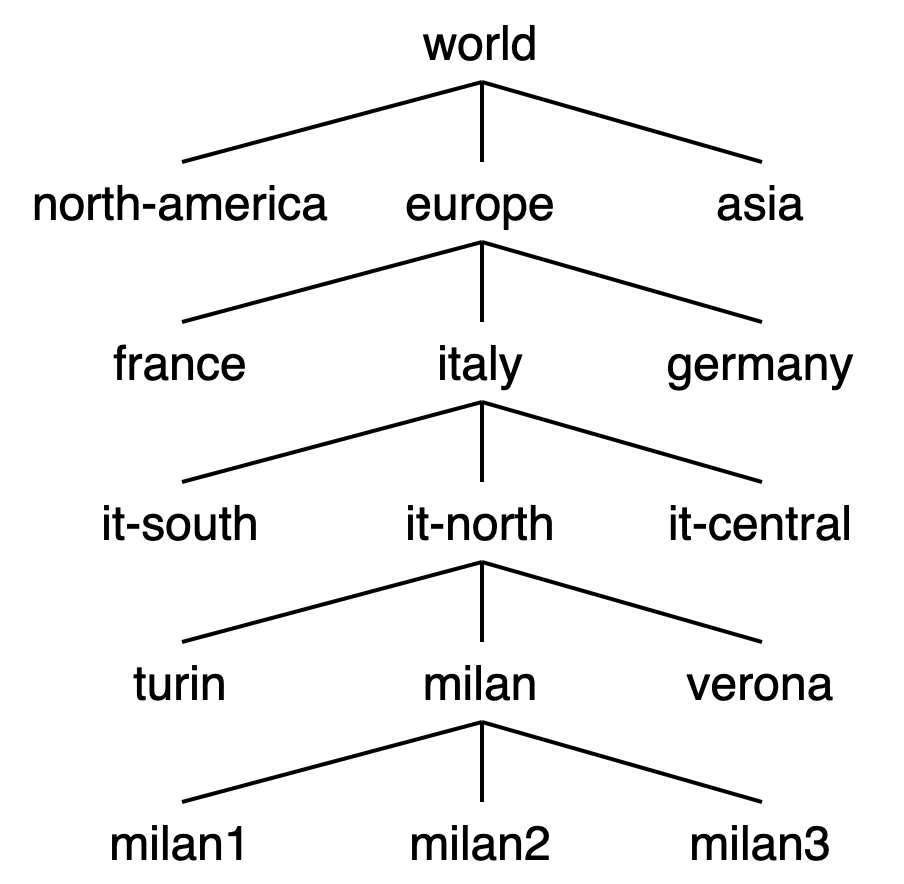
\includegraphics[width=5.5cm]{Figures/Solution/hierarchy.png}
\end{wrapfigure} 

To allow flexibility in the deployments and, as we will see later, to allow geographical aggregations we can organize the various machines running in the data centers and cloudlets in a hierarchy with multiple levels.
In Figure \ref{fig:hierarchy} we reported an example: we first have a division by continent (or large regions), then by country, territory, city and district.
Note that each element in the hierarchy should not necessarily be a different data center: a big data center in Milan can be both a receiver for "city" and "country" deployments/aggregations.
\vspace{0.5cm}


\subsection{Specifying Locations}
The job of specifying the available locations should be responsibility of the web infrastructure company, but still the developer may want to customize the arrangement or may want to use their personal infrastructure. 

So we must provide a way to specify the hierarchy, we chose to implement the API in the following way:
\begin{itemize}
    \item Levels: the list of levels characterized by their identifiers (e.g., "continent", "country", "territory", "city", "district");
    \item Hierarchy: a way to specify the hierarchy, starting from the uppermost level and going down to the lowest level. Each level can contain multiple locations, and each location will aggregate data of the relative area;
    \item Location: each location must be associated to an entry point that defines the actual cloudlet or data center to be used (so for the location there must be defined gateway, port and password).
\end{itemize}

TODO show constraints


\subsection{Specifying Deployments}
Now that we have the hierarchy specified we can use this hierarchy to make a powerful deployment API. The developer should be able to deploy on a specific level of the hierarchy only in a certain area and to exclude a specific subsection from this area.

To allow such deployment we established the following concepts:
\begin{itemize}
    \item \inlinecode{inEvery}: a string representing the level on which to deploy the function.
    \item \inlinecode{inAreas}: a list of string of areas, specifying in which areas to deploy. If unspecified we can assume the developer wants it deployed on every area of the level specified in \inlinecode{inEvery}. 
     \item \inlinecode{exceptIn}: a list of string of areas, that are an exception to what previously defined before. In these areas the developer does not want to perform the deployment.
\end{itemize}

\begin{example}
Deploy on every district worldwide.
Becomes:
\begin{itemize}
    \item \inlinecode{inEvery}: "district"
    \item \inlinecode{inAreas}: [ ]
    \item \inlinecode{exceptIn}: [ ]
\end{itemize}
\end{example}

\begin{example}
Deploy on every city in Europe and Asia, excluding the cities in Italy and excluding the city of Tokyo.
Becomes:
\begin{itemize}
    \item \inlinecode{inEvery}: "city"
    \item \inlinecode{inAreas}: ["europe", "asia"]
     \item \inlinecode{exceptIn}: ["italy", "tokyo"]
\end{itemize}
\end{example}

\begin{example}
Deploy on every district in Europe and India, excluding the districts in France and excluding the districts in Milan.
Becomes:
\begin{itemize}
    \item \inlinecode{inEvery}: "district"
    \item \inlinecode{inAreas}: ["europe", "india"]
     \item \inlinecode{exceptIn}: ["france", "milan"]
\end{itemize}
\end{example}

In the examples we saw that the developer should also be allowed to mix the levels of the areas specified, using different levels of the hierarchy inside the \inlinecode{inAreas} and \inlinecode{exceptIn} lists.

TODO show constraints


\section{Managing Limited Resources}
Edge locations have limited resources compared to central data centers, so web infrastructure companies have to work around the limitations in order to provide a reliable service.
Due to these limitations, Function-as-a-Service (FaaS) is the current de facto standard for companies that provide computing resources at the edge to the public. Examples of services are AWS Lambda@Edge (an evolution of the famous AWS Lambda service on the cloud) \cite{aws-lambda-at-edge} or Cloudflare Workers \cite{cloudflare-workers}. It can be easily understood that providing Infrastructure-as-a-Service (IaaS) or Platform-as-a-Service (PaaS) to the public on the limited resources available at the edge is clearly less efficient for companies.

Therefore we decided to use in our framework the FaaS paradigm as a way to allow the users of the framework (the developers) to perform computation on the edge. The developer, should also be able to specify the Random Access Memory (RAM) allocated for the function. The default allocated memory can be a low value, but if there is a more complex function requiring additional memory usage the developer can change the allocated memory (the web infrastructure company can then charge more based on the memory requested).

But resources are not only limited in the sense of computation, also storage resources are limited on the edge. To take into account the aforementioned issue we decided to use a key-value database for the stateful part of our approach. A key-value database allows us to perform extremely efficient (but simple) queries, and is perfect for the limited resources available on the edge. To avoid to accumulate data we also introduced in our framework a Time-To-Live (TTL) which the developer must specify. For example with a TTL of 5 days, after making a write to the database the data, if not updated, can be deleted after 5 days.


\subsection{Writing Data}
Our goal is to provide the developers an easy way to create geographical aggregations of data. If for the data it does not make sense to create geographical aggregations then it would make more sense to use a core-centric approach to manage this data. In our approach by having the data geographically distributed it means that those data correspond to information coming from the respective geographic area.

Furthermore in Chapter \ref{ch:problem_formulation} we outlined use cases which are static in the sense of location, or for which having discontinuity in the data is not a problem. Therefore we decided to not introduce any session consistency to avoid the cost of managing such sessions: heavy communications between the locations. This means that if we are performing a "city" aggregation and a client that is sending data is currently travelling and changes its position to a new "city" area, then its old data will remain in the previous "city" area and will not transferred to the new one.

To manage such conditions our approach should have the following properties:
\begin{itemize}
    \item Write Action: the action to perform for writing data (e.g., set, add to list, ...)
    \item Key: The key that will be associated to the value as in a standard key-value database.
     \item Data: the data to be associated to the key (so it can be then obtained from the key) or the data to be added to the list specified by the key.
     \item Referring Area Level: the highest level on which to aggregate the data.
     \item Should Save In Intermediate Levels: a true or false property that if set to true saves the data only in the level specified by the Referring Area Level, otherwise the data is saved on the receiving level and on all the other upper levels, up until the level specified by Referring Area Level.
     \item Time To Live: limits the lifespan of the data.
\end{itemize}

To provide some examples, we see a few write calls that a developer can make:

\begin{example}
The developer makes the following write call on a function deployed at the "city" level:
\begin{itemize}
    \item Write Action: set
    \item Key: mykey1
    \item Data: data1
    \item Referring Area Level: continent
    \item Should Save In Intermediate Levels: false
    \item Time To Live: 10 days
\end{itemize}
The framework will save the data only at the continent level (so if the code is executed in the "milan" location, the data will be saved in the "europe" location). The framework will create (or update) key "mykey1" with the value "data1" and will set a lifespan of the data to 10 days.
\end{example}

\begin{example}
The developer makes the following write call on a function deployed at the "city" level:
\begin{itemize}
    \item Write Action: set
    \item Key: mykey2
    \item Data: data2
    \item Referring Area Level: continent
    \item Should Save In Intermediate Levels: true
    \item Time To Live: 30 days
\end{itemize}
The framework will save the data at the continent, country, territory and city levels (so if the code is executed in the "milan" location, the data will be saved in the "it-north", "italy" and "europe" locations). In each of these locations the framework will create (or update) key "mykey2" with the value "data2" and will set a lifespan of the data to 30 days.
\end{example}

\begin{example}
The developer makes the following write call on a function deployed at the "city" level:
\begin{itemize}
    \item Write Action: add to list
    \item Key: mylist1
    \item Data: data1
    \item Referring Area Level: country
    \item Should Save In Intermediate Levels: false
    \item Time To Live: 1 day
\end{itemize}
The framework will save the data only at the continent level (so if the code is executed in the "milan" location, the data will be saved in the "italy" location). The framework will add to the list associated to the key "mylist1" the value "data1" and will set a lifespan to the single element of the list to 1 day.
\end{example}


\subsection{Reading Data}
As we have seen the developer has to think carefully how to handle the writing of the data with the objective to partition geographically the data. But after data have been thoughtfully partitioned then the reading of the data is instantaneous.
When running the code in a certain location, by specifying only the reading action and the key, the framework obtains the data present in the location and associated to that key.

So only the following two properties are use for making reads:
\begin{itemize}
    \item Read Action: the action to perform for reading data, "get" to obtain the single value from the key saved with "set", "get list" to obtain all the values saved with "add to list".
    \item Key: The key of the value or the list to be read.
\end{itemize}

\begin{example}
The developer makes the following read call on a function deployed at the "continent" level:
\begin{itemize}
    \item Read Action: get
    \item Key: mykey1
\end{itemize}
The framework will obtain the value associated to the key "mykey1" if present and if not expired due to the TTL.
\end{example}

\begin{example}
The developer makes the following read call on a function deployed at the "country" level:
\begin{itemize}
    \item Read Action: get list
    \item Key: mylist1
\end{itemize}
The framework will obtain all the not expired elements contained in the list associated to the key "mylist1".
\end{example}


\section{Applying the Solution to Use Cases}
\label{sec:solution_use_cases}
In this section we show how the solution we thought can be applied to some of the use cases we presented in Chapter \ref{ch:problem_formulation}.


\subsubsection{IoT Data Compression}
In this use case we try to compress the data of IoT sensor by sending only significant value changes, this concept can be applied for example to a temperature sensor where the value can be pretty much equal for very long periods of time.

We can implement this use case by having a stateful function that checks whether the new value is equal or almost equal to the previous value.

With our solution a possible execution can be the following:
\begin{example}
Deployment:
\begin{itemize}
    \item \inlinecode{inEvery}: "building"
    \item \inlinecode{inAreas}: [ "factory1", "factory2" ]
    \item \inlinecode{exceptIn}: [ ]
\end{itemize}
With this deployment we are deploying a function in every location at the "building" level.

Reads:
\begin{itemize}
    \item Read Action: get
    \item Key: sensor1
\end{itemize}
Here we read the previous value of "sensor1" and we can compare it to the value sent by the sensor, if it differs substantially the function can forward the value to the cloud or can also fire an alert.

To update the value stored in the stateful support of the function we do the following write action:
\begin{itemize}
    \item Write Action: set
    \item Key: sensor1
    \item Data: <<value sent by the sensor>>
    \item Referring Area Level: building
    \item Should Save In Intermediate Levels: false
    \item Time To Live: 5 days
\end{itemize}
This stores the value locally in the location where the code is deployed, since the function has been deployed to the "building" level and the Referring Area Level is the same "building" level.
\end{example}


\subsubsection{Road Traffic Monitoring}
In this use case we analyze video footage data to get an insight on the road traffic and then use such insight in an algorithm to find the fastest path between two points.

We can implement this use case with two functions: the first function receives the data from the cameras, converts the footage in a value of traffic and finally saves this value; while the second function computes the fastest path between two points by using the information of the traffic saved by the first function.

Therefore the first function can work like this
\begin{example}
Deployment:
\begin{itemize}
    \item \inlinecode{inEvery}: "district"
    \item \inlinecode{inAreas}: [ "us" ]
    \item \inlinecode{exceptIn}: [ ]
\end{itemize}
With this deployment we are deploying a function in every location at the "district" level in the area corresponding to the United States.

Writes:
\begin{itemize}
    \item Write Action: set
    \item Key: <<camera ID>>
    \item Data: <<value of traffic computed from footage>>
    \item Referring Area Level: central
    \item Should Save In Intermediate Levels: true
    \item Time To Live: 30 minutes
\end{itemize}
With this database action that we are performing at the "district" level (since the function is deployed at the "district" level) we are saving data in the key that corresponds to the camera that sent the input. We are using a low TTL value since if the camera goes offline and does not provide an update, then we can consider the value stored to not be reliable after 30 minutes.
We are saving the value with Referring Area Level "central" and also saving in intermediate levels, this means that every level in between "district" and "central" (both also included) will have a copy of the data.
\end{example}

The second function instead can be deployed at multiple levels and can work in the following way:
\begin{example}
Reads:
\begin{itemize}
    \item Read Action: get
    \item Key: <<camera ID>>
\end{itemize}
This read action can be performed for multiple camera IDs depending on the possible paths that can be taken between the two points.
By having the information of the traffic an algorithm can be created to compute which path is likely faster. 
\end{example}


\subsubsection{Trending Topics}
In this use case we want to find the trending topics in a certain region in an application (like trending user in a social network, or trending searches).

We can divide the implementation of this use case in two parts: a first part where we aggregate the data of the topics per region; and a second part that periodically finds the trending topics from the raw data.

We may also want to aggregate this data with different granularities: "city", "territory", "country".

So with our solution a possible execution for the first part can be the following:
\begin{example}
Deployment:
\begin{itemize}
    \item \inlinecode{inEvery}: "city"
    \item \inlinecode{inAreas}: [ ]
    \item \inlinecode{exceptIn}: [ ]
\end{itemize}
With this deployment we are deploying a function in every location at the "city" level.

Writes:
\begin{itemize}
    \item Write Action: add to list
    \item Key: trending-topics
    \item Data: <<topic seen or searched by the client>>
    \item Referring Area Level: country
    \item Should Save In Intermediate Levels: true
    \item Time To Live: 2 days
\end{itemize}
With this database action that we are performing at the "city" level (since the function is deployed at the "city" level) we are adding data to the list of "trending-topics". The Referring Area Level is "country" so the data will be aggregated to the "country" level, but since we are also saving in intermediate locations this data will be also sent to the respective "territory" location and saved locally in the current "city" location.

We make an example with actual names to be more clear: a client is searching the topic "My search" and the client is located in the city of Milan. This client send this topic to the deployed function, the function has been deployed at the "city" level so it will be executed in a data center in Milan. This function executing in Milan can perform a pre-process on the input (e.g., making it lowercase) and then adds the input to the list "trending-topics". The write is performed with Referring Area Level "country" but also saved in intermediate locations, therefore the input will be forwarded to the respective "country" location (in this case a data center that refers to the Italy area), to the "territory" location (in this case a data center that refers to the Northern region of Italy) and also saved locally in the data center in Milan.
\end{example}

While a possible execution for the second part of finding the trending topics (in this case the trending topics of the territory) can be the following:
\begin{example}
Deployment:
\begin{itemize}
    \item \inlinecode{inEvery}: "territory"
    \item \inlinecode{inAreas}: [ ]
    \item \inlinecode{exceptIn}: [ ]
\end{itemize}
With this deployment we are deploying a function in every location at the "territory" level.

Reads:
\begin{itemize}
    \item Read Action: get list
    \item Key: trending-topics
\end{itemize}
With this database action that we are performing at the "territory" level (since the function is deployed at the "territory" level) we are reading all the non-expired data in the list "trending-topics". In our case this list contains all the topics searched by the users in the last 2 days in the respective "territory" area where this function is executed. This function can then be executed periodically to update the trending topics.

Since the list is obtained in its entirety the trending algorithm can be anything the developer prefers (e.g., most-frequent analysis, derivative of the frequency, etc...).
\end{example}

